\chapter{Additional Files and Schematics}
\label{ch_appendixa}

%Add any information here that you would like to have in your project but is not necessary in the main
%text. Remember to refer to it in the main text. Separate your appendices based on what they are for
%example. Equation derivations in Appendix A and code in Appendix B etc.

\lstinputlisting[caption={Optimized Goertzel Algorithm - Octave Function\label{lst:optimized_goertzel_algorithm}}]{../goertzel/hc_calculate_goertzel.m}

\lstinputlisting[caption={Frequency Response Test - Octave Script\label{lst:frequency_response_script}}]{../goertzel/test_goertzel.m}

\begin{figure}[H]
	\centering
	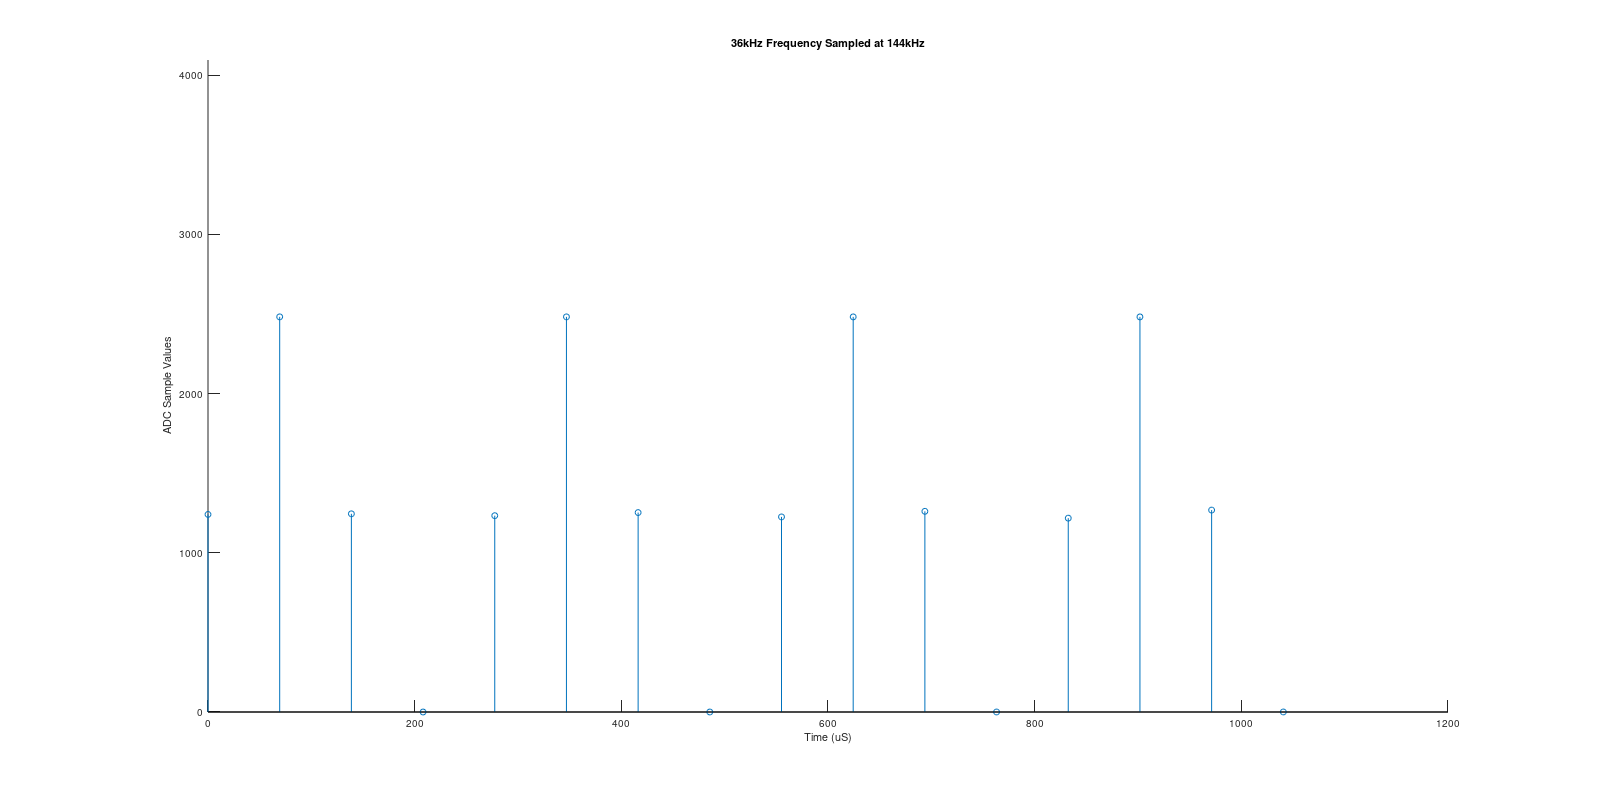
\includegraphics[width=\linewidth]{figures/results/36khz_frequency.png}
	\caption{Plot of sampled 36kHz sinusoid}
	\label{fig:sampled_36khz_sinusoid}
\end{figure}